\section{Software Architektur}

\subsection{Services \& Komponenten}

Insgesamt gibt es 4 Microservices und ein Gateway. In den folgenden Unterkapiteln werden die Microservices  und das Gateway genauer beschrieben.

\subsubsection{Gateway}

Die Aufgabe des Gateways ist es Eingehende Anfrage außerhalb des Clusters basierend aufgrund von Routing regeln weiterzuleiten. Darüber hinaus findet sich am Gateway auch die Zentrale Swagger UI Dokumentationsplattform auf der die Endbenutzer die Exposed Rest Schnittstellen der Microservices ansehen können (bzw. die Dokumentation lesen können).

\subsubsection{Entity-Service}

Die Aufgabe des Entity-Services ist es die Metadatan und statischen Daten der Entitäten der Akteuren (Autos und Ampeln) zu verwalten. Die Akteure registrieren sich bei diesem Service um teil der Simulation zu werden. Über verschiedene Rest Schnittellen kann können diese Daten dann abgefragt werden.

\subsubsection{Tracking-Service}

Die Aufgabe des Tracking-Services ist es die dynamischen Daten der Entitäten der Akteuren (Autos und Ampeln) zu verwalten. Während der Simulation werden diese Daten an das Tracking-Service geliefert und dieses Persistiert diese. Über verschiedene Rest Schnittellen kann können diese Daten dann abgefragt werden.

\subsubsection{Simulator-Service}

Die Zentrale Aufgabe des Simulator-Services ist es die Simulation zu starten und zu beenden. Sobald die Simulation gestartet wird, simuliert dieses Service Ampeln und Fahrzeuge. Es registriert diese Akteure und spielt das Verhalten, welches im Algorithmus spezifiziert wurde, ab.

\subsubsection{Flowcontrol-Service}

Das Flowcontrol-Service hat zur Aufgabe anhand von dem aktuellen Stand eines Fahrzeuges die optimale Geschwindigkeit zu berechnen, sodass eine grüne Phase erreicht wird. 

\subsection{Schnittstellen \& Kommunikation der Services}

\begin{figure}[h]
	\centering
	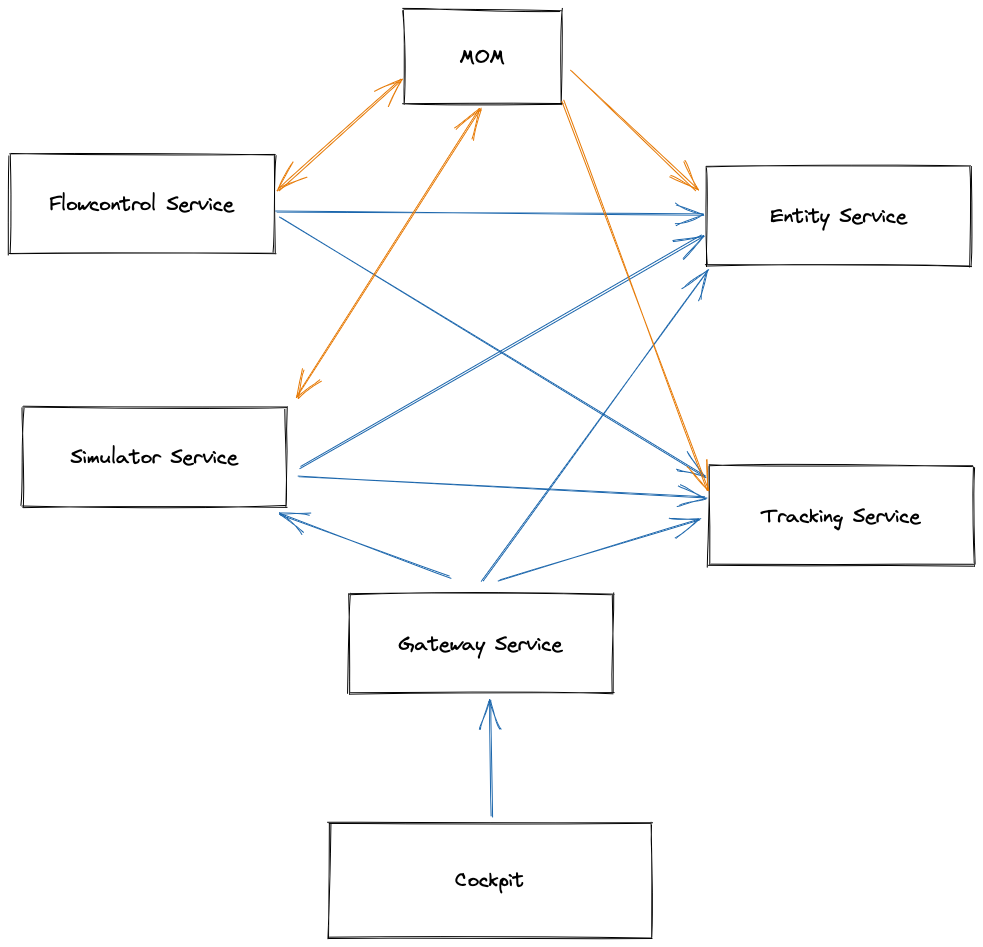
\includegraphics[width=1\textwidth]{./figures/whole_system_communication.png}
	\caption{Übersicht aller Schnittstellen und Kommunikationen}
	\label{fig:wholesystem_view}
\end{figure}

Wie man der Abbildung \ref{fig:wholesystem_view} entnehmen kann, finden sich innerhalb unseres Systems 2 Arten von Schnittstellen. Zuerst gibt es die konventionelle Synchrone Schnittstelle nämlich REST (in Abbildung \ref{fig:wholesystem_view} mittels blauen Pfeilen dargestellt) und weiteres die Asynchrone Schnittstelle (in Abbildung \ref{fig:wholesystem_view} mittels orangen Pfeilen dargestellt), welche mittels einer Message Oriented Middleware (in diesem Falle RabbitMQ) realisiert wurde.
Grundsätzlich verwenden wir asynchrone Kommunication damit Kommunikation, welche häufig erfolgt, nicht die Services blockiert und synchrone für Operationen, die nicht Zeitkritisch sind bzw. asynchron nicht viel Sinn machen würde.

\subsubsection{REST}

\begin{figure}[h]
	\centering
	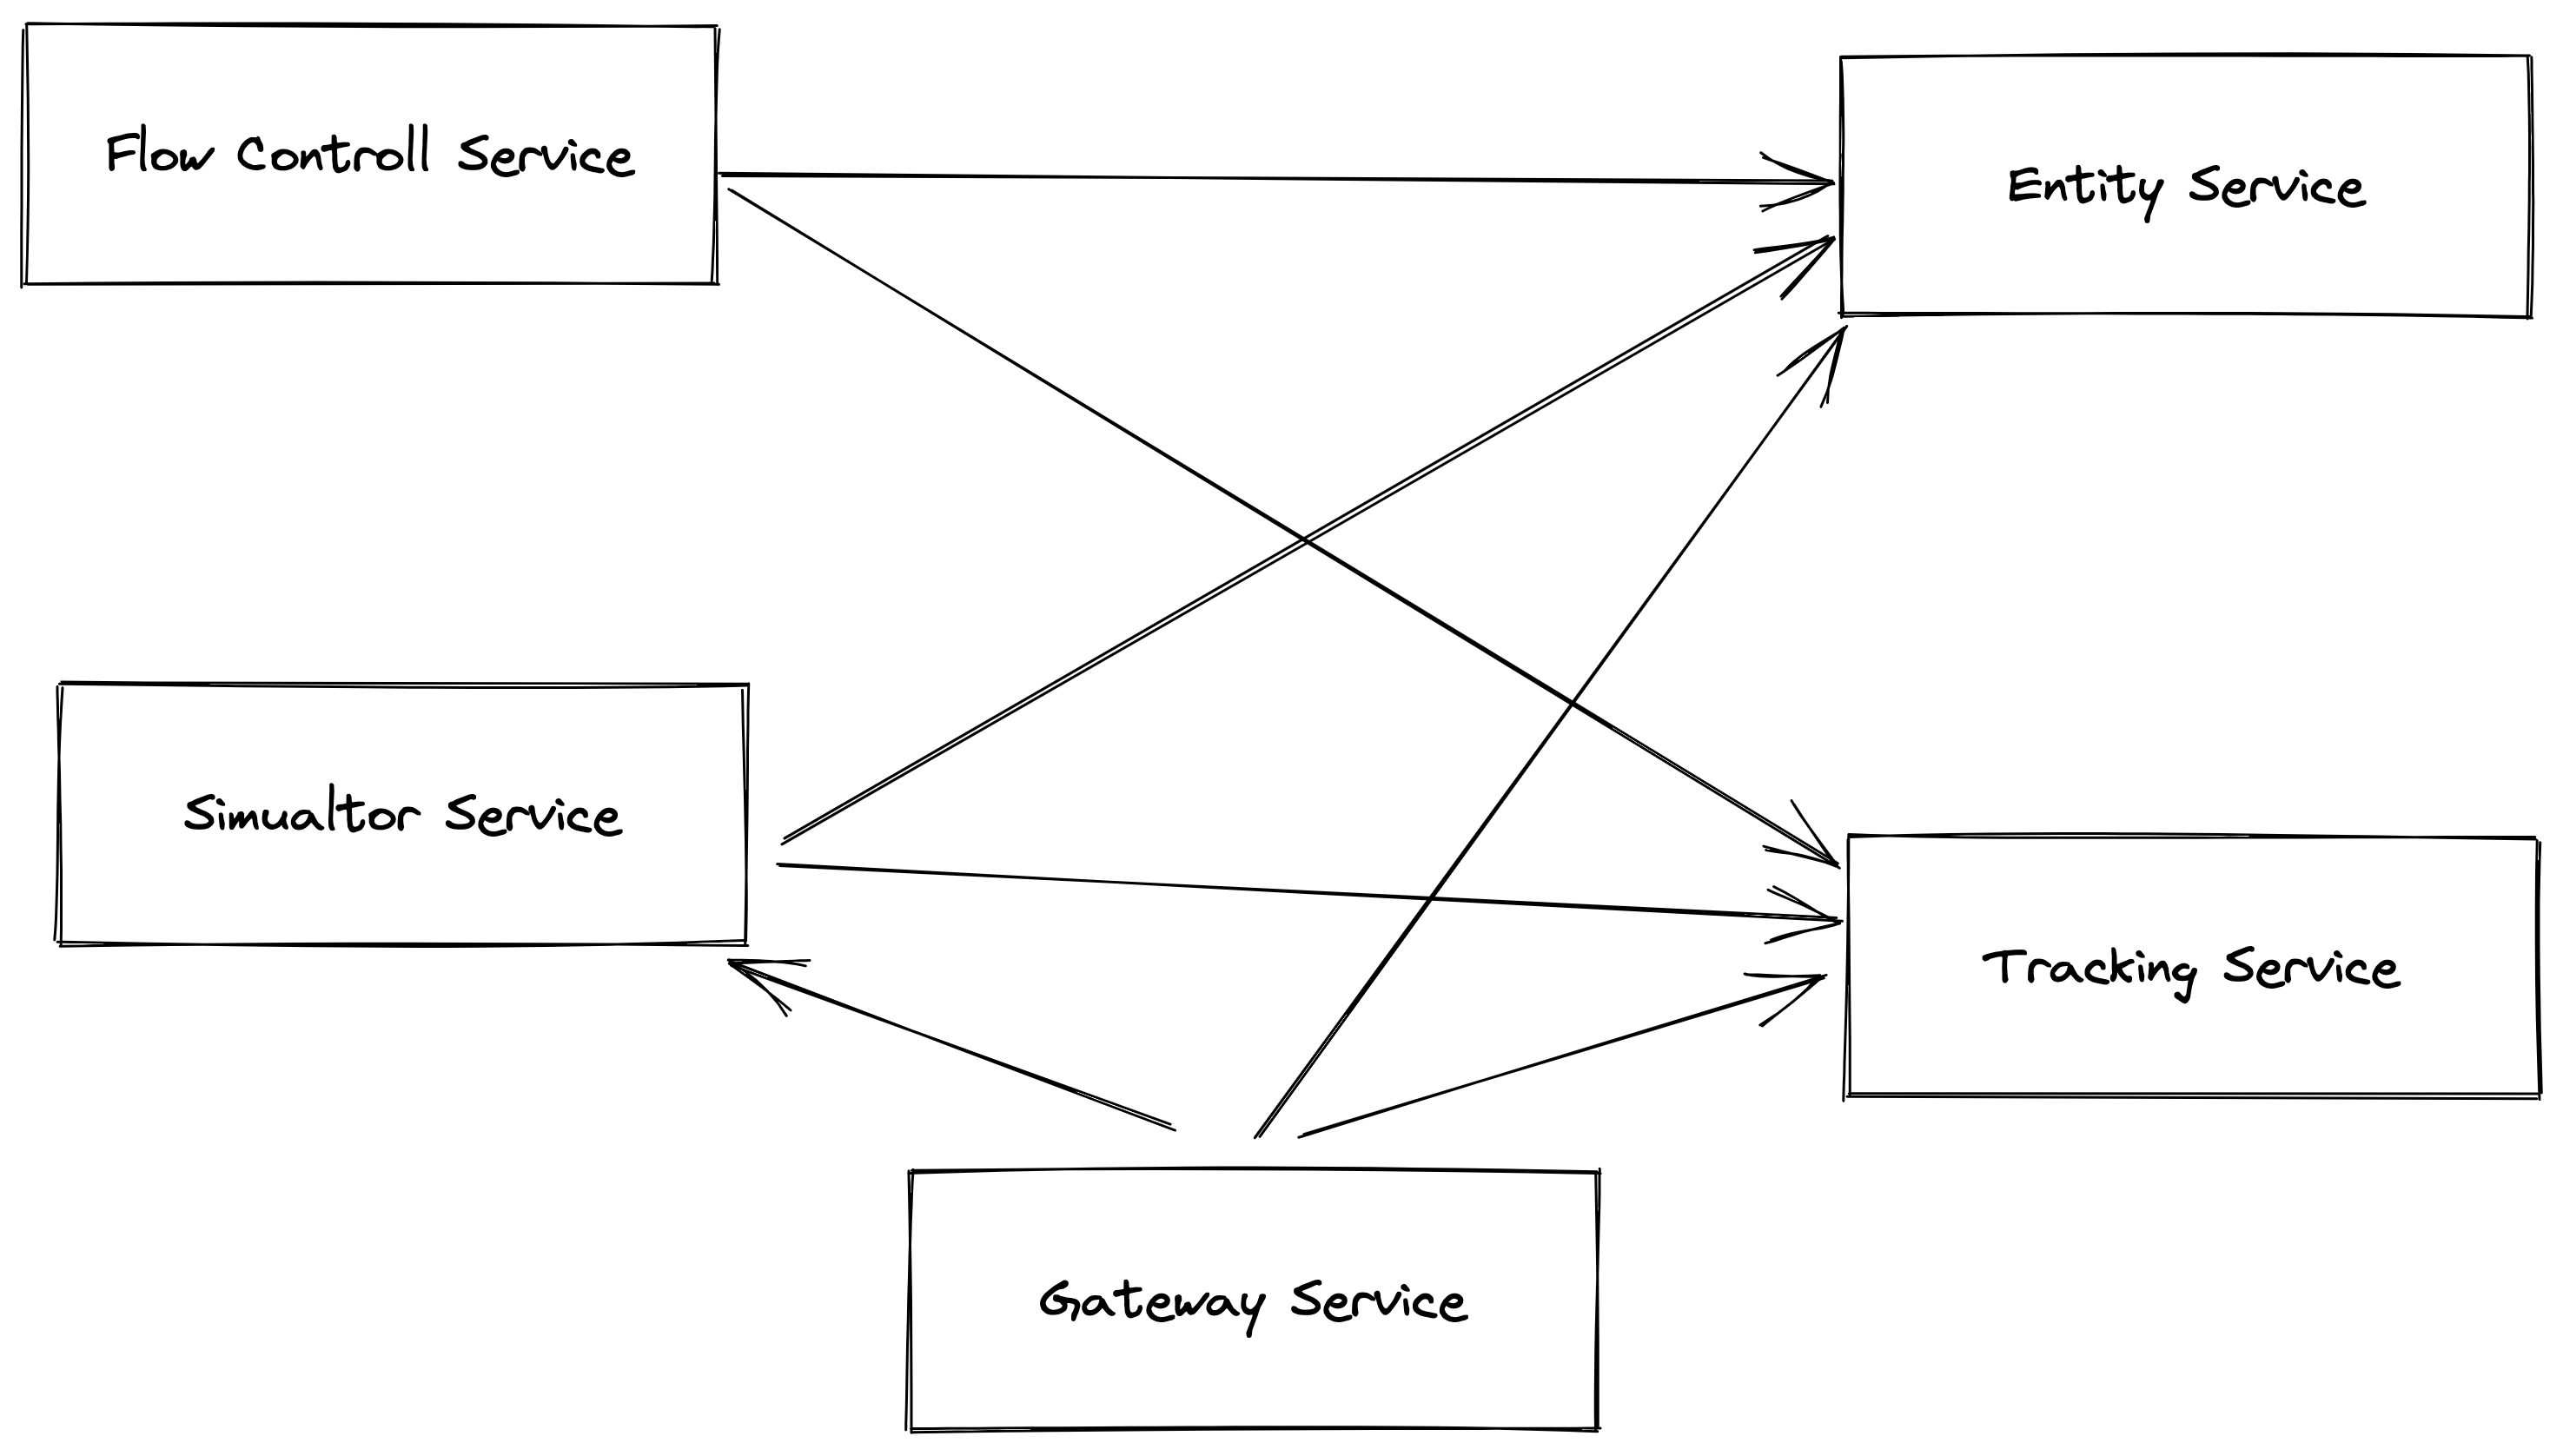
\includegraphics[width=1.02\textwidth]{./figures/rest_communication.png}
	\caption{Überblick der Rest Kommunikation}
	\label{fig:kom_rest_overview}
\end{figure}

In der Abbildung \ref{fig:kom_rest_overview} kann man einen Überblick der REST Kommunikation der Services sehen. 

\paragraph{Gateway}
Auf dem ersten Blick kann man sofort erkennen, dass das Gateway aufgrund seiner Zielfunktionalität mit allen Services kommuniziert, welche eine REST Schnittstelle besitzen und diese auch nach außen zugänglich machen wollen.

\paragraph{Flowcontrol-Service}
Wichtig ist hier hervorzuheben, dass das Flowcontrol-Service keine REST Schnittstelle bereitstellt für andere Services. Dieses Service kommuniziert mit dem \textit{Entity-Service} und dem \textit{Tracking-Service} damit alle Eingaben für den Algorithmus zur Berechnung der Optimal Geschwindigkeit angefragt werden können.

\paragraph{Simulator-Service}
Das Simulator-Service stellt insgesamt 3 REST Endpunkte zur verfügung, die für das starten/stoppen der Simulation gebraucht werden. Das Simulator-Service kommuniziert mit dem \textit{Entity-Service} und dem \textit{Tracking-Service} um einen Stoppen bzw. Reset der Simulation zu erwirken.

\paragraph{Entity-Service}
Das Entity-Service stellt einige REST Endpunkte zur Verfügung um die Daten der Akteure in der Simulation abfragen zu können. Das Entity-Serivce selbst stellt niemals anfragen an andere Services im System.

\paragraph{Tracking-Service}
Das Entity-Service stellt einige REST Endpunkte zur Verfügung um den Stand der Akteure in der Simulation abfragen zu können. Das Tracking-Serivce selbst stellt niemals anfragen an andere Services im System.

\subsubsection{Message Oriented Middleware}

\begin{figure}[h]
	\centering
	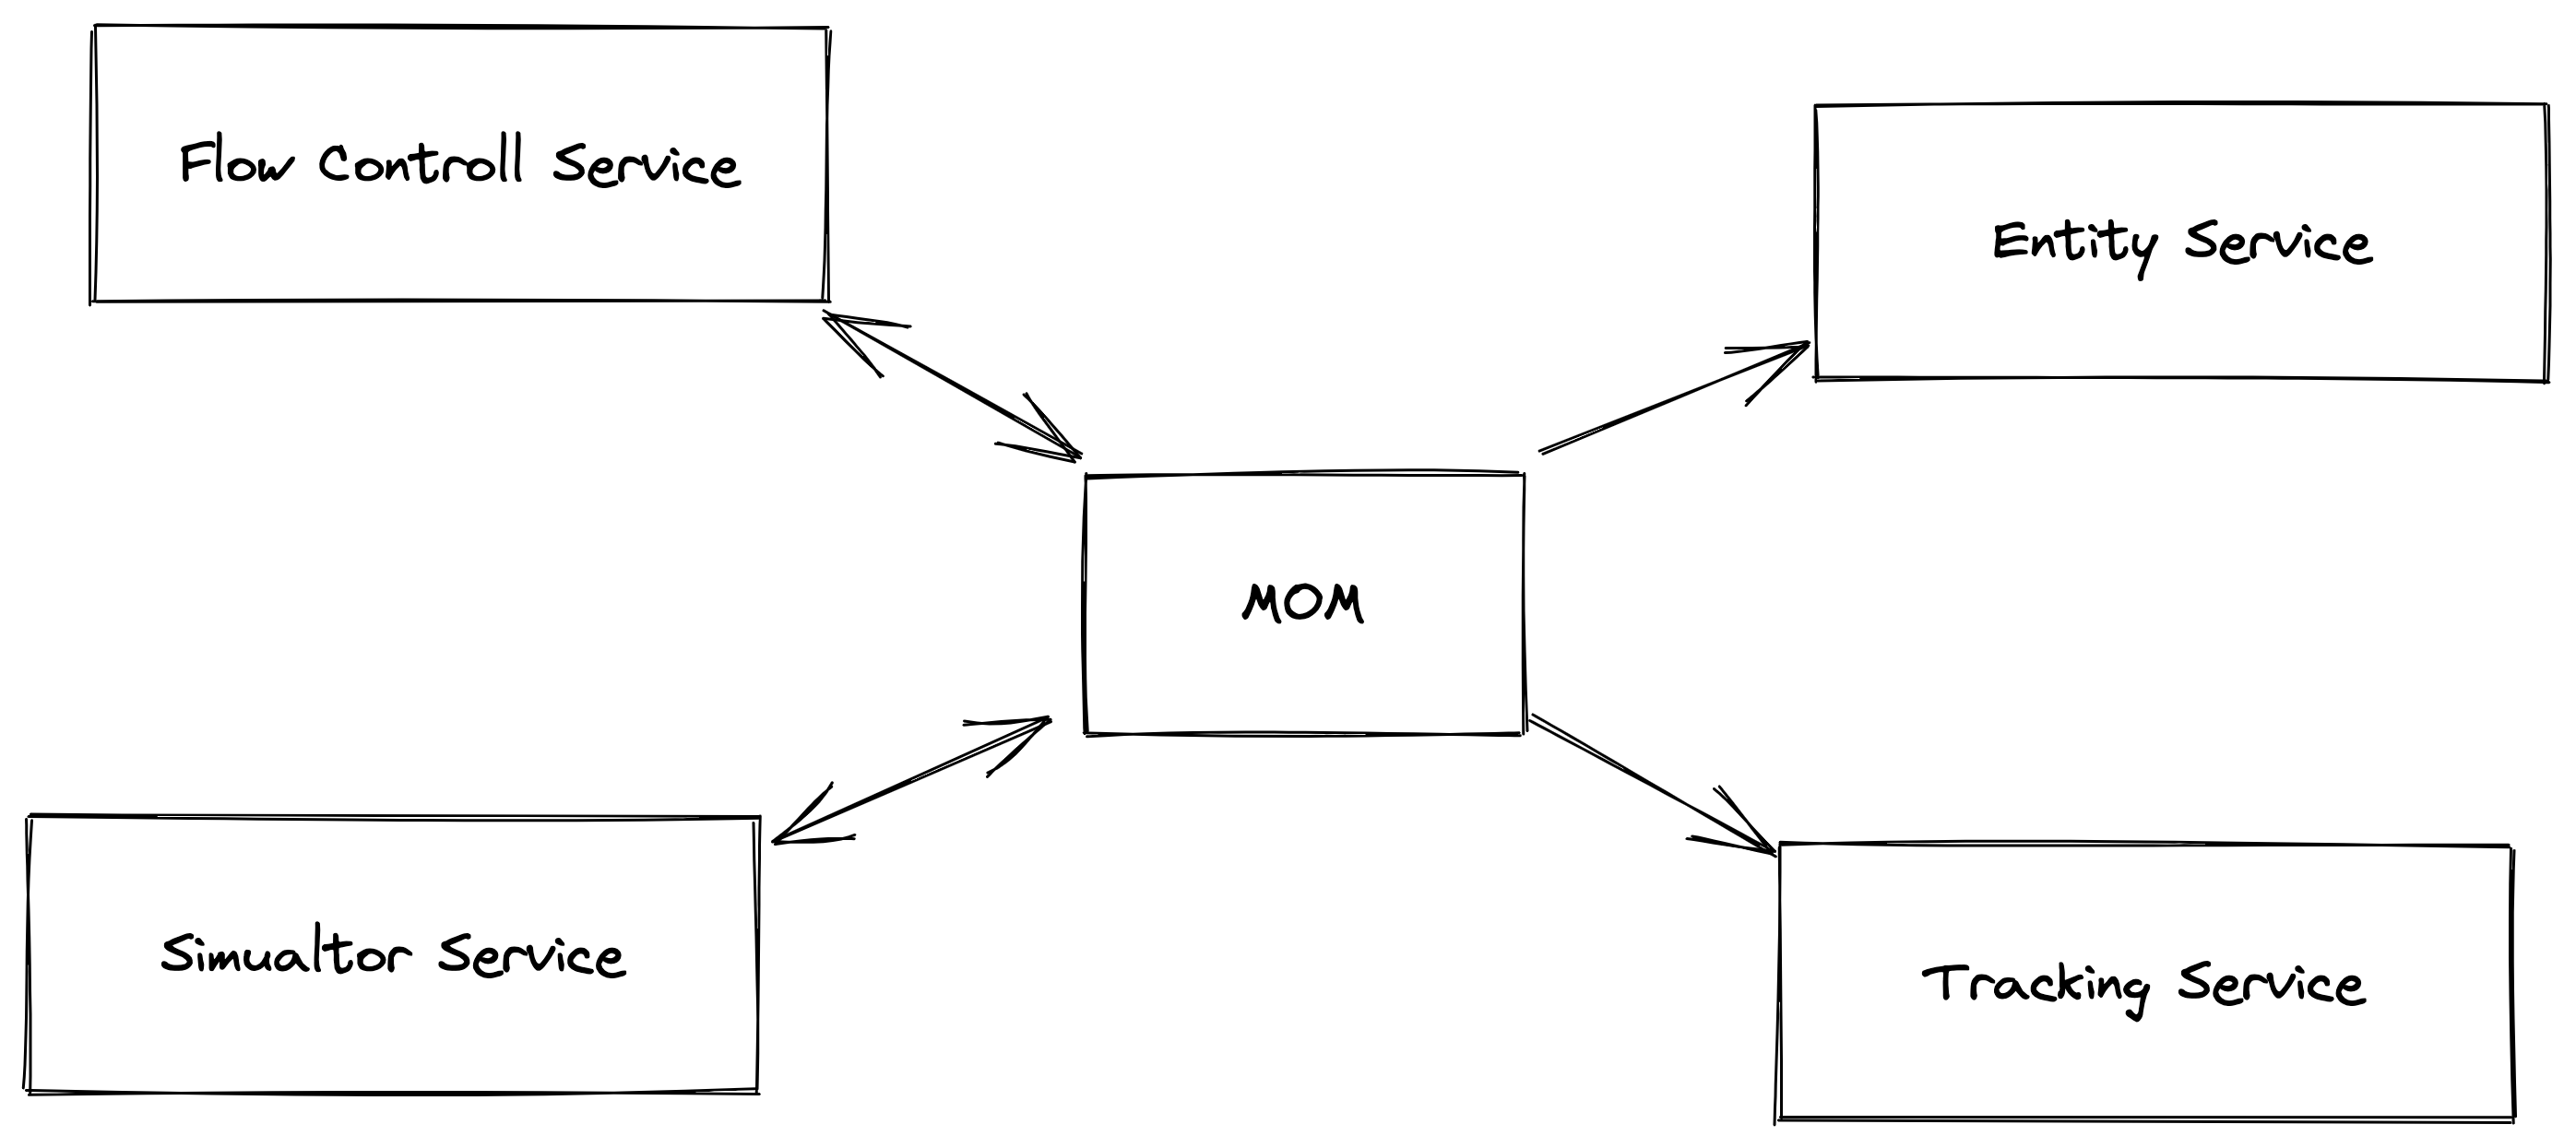
\includegraphics[width=1.02\textwidth]{./figures/mom_communication.png}
	\caption{Überblick der MoM Kommunikation}
	\label{fig:kom_mom_overview}
\end{figure}

In der Abbildung \ref{fig:kom_mom_overview} kann man einen Überblick der MoM Kommunikation der Services sehen. Wie in der Abbildung zu sehen ist, empfangt das \textit{Tracking-Service} und das \textit{Entity-Service} nur Daten von der MoM und senden keine zu ihr. Auf der anderen Seite sieht man dass das \textit{Flowcontrol-Service} und \textit{Simulator-Service} Daten an die MoM senden und empfangen. 

Insgesamt gibt es sechs Queues und eine Fanout-Exchange (mit dem Namen \verb|fanout.carState|).
Die Namen der Queues sind wie folgt: 
\begin{enumerate}
	\item \verb|car-state-tracking| 
	\item \verb|car-state-flow| 
	\item \verb|car| 
	\item \verb|traffic-light| 
	\item \verb|traffic-light-state| 
	\item \verb|car-speed| 
\end{enumerate}

In den folgenden Paragraphen werden wir uns ansehen wie die Queues und die Fanout-Exchange verwendet werden.

\begin{figure}[h]
	\centering
	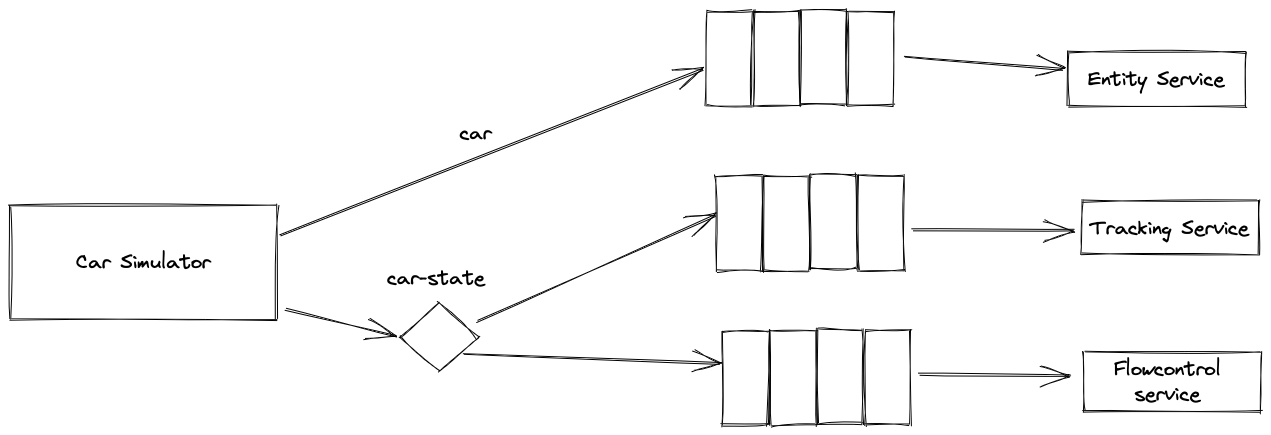
\includegraphics[width=1\textwidth]{./figures/car_simulator_mom.png}
	\caption{Verwendung der \textit{Car}, \textit{Car-State-*} und Exchange}
	\label{fig:car_simulator_mom}
\end{figure}

\paragraph{car, car-state-*, exchange}
In Abbildung \ref{fig:car_simulator_mom} sieht man die Verwendung der Queues \textit{Car}, \textit{Car-State-*} und der Exchange. Am Anfang der Simulation sendet der \textit{Car-Simulator} an die Queue \textit{car} die Informationen für die Registrierung des Fahrzeuges. Diese Queue wird vom Entity-Service konsumiert. Während der Simulation wird die aktuelle Position, Geschwindigkeit und weiteres dynamische Daten an die Fanhout-Exchange gesendet (welche in der Abbildung \ref{fig:car_simulator_mom} als Raute gekennzeichnet ist). Die Fanout-Exchange leitet diese dann an die beiden Queues \textit{car-state-flow} und \textit{car-state-tracking} weiter. Diese Design Entscheidung wurde getroffen, da es sich hier um ein PubSub Szenario handelt und nicht einem Competing-Consumer.

\begin{figure}[h]
	\centering
	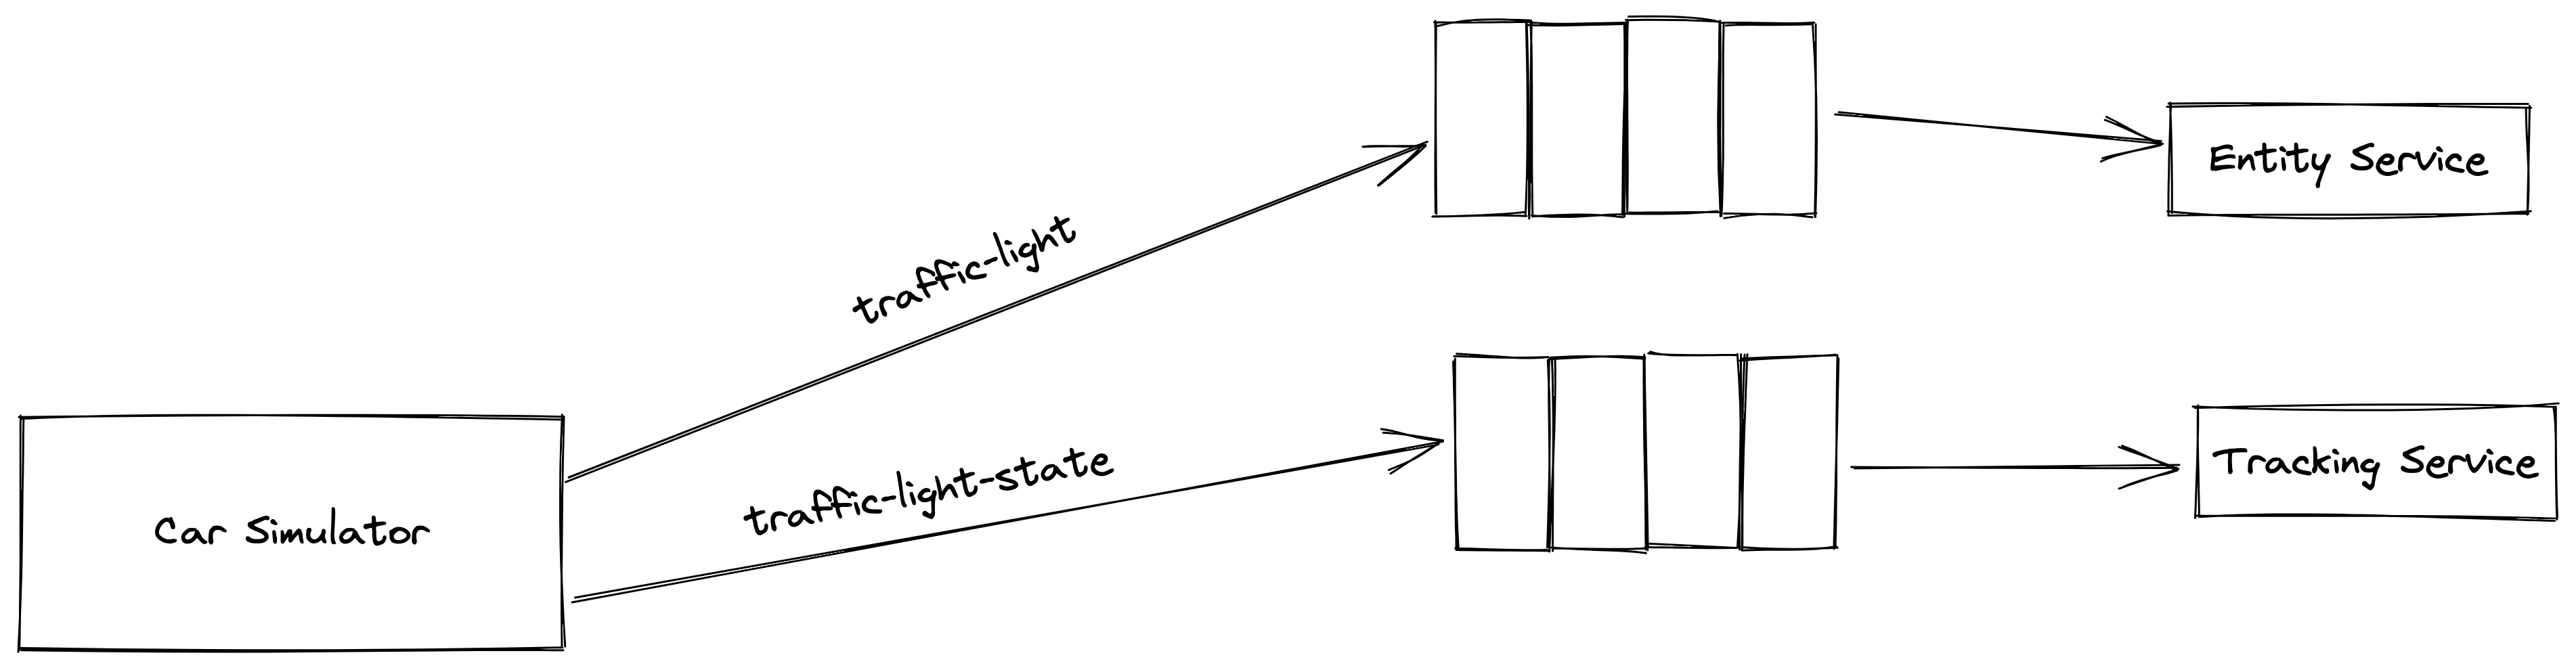
\includegraphics[width=1\textwidth]{./figures/traffic-light_simulator_mom.png}
	\caption{Verwendung der Queues \textit{traffic-light}, \textit{traffic-light-state} }
	\label{fig:light_simulator_mom}
\end{figure}

\paragraph{car, car-state-*, exchange}
In Abbildung \ref{fig:light_simulator_mom} sieht man die Verwendung der Queues \textit{traffic-light}, \textit{traffic-light-state}. Am Anfang der Simulation sendet der \textit{TrafficLight-Simulator} an die Queue \textit{traffic-light} die Informationen für die Registrierung der Ampel. Diese Queue wird vom Entity-Service konsumiert. Während der Simulation wird die verbleibende Zeit im State und weitere dynamische Daten an die Queue \textit{traffic-light-state} gesendet, welceh vom \textit{tracking-service} konsumiert wird.

\begin{figure}[h]
	\centering
	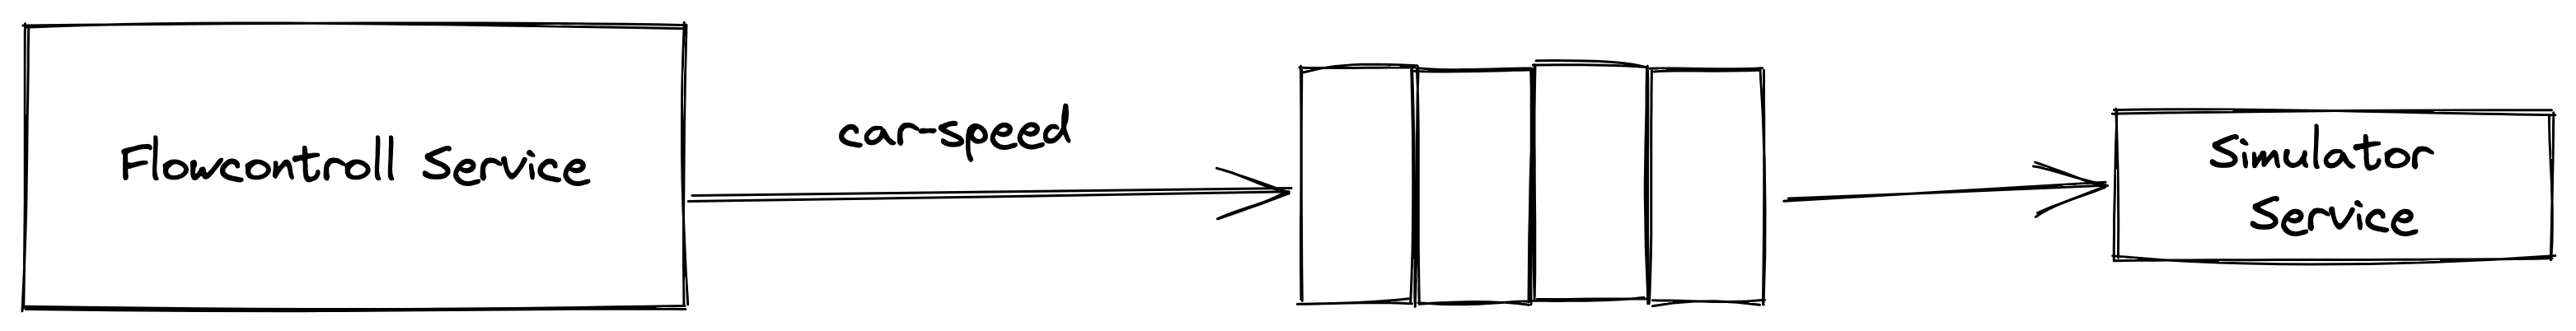
\includegraphics[width=1\textwidth]{./figures/flow_controll_speed_mom.png}
	\caption{Verwendung der Queue \textit{car-speed}}
	\label{fig:car_speed_mom}
\end{figure}

\paragraph{car-speed}
In Abbildung \ref{fig:light_simulator_mom} sieht man die Verwendung der Queue \textit{car-speed}. Das \textit{Flowcontrol-Service} sendet nachdem die optimale Geschwindigkeit berechnet wurde, diese mittels der Queue \textit{car-speed} and das \textit{Simulator-Service}.